
The flow behind a circular cylinder started impulsively in rotation and/or translation is investigated as a prototype of unsteady separated flows.
Despite of the seeming simplicity of this problem, the flow evolves with non-trivial vortex shedding, in which one outgoing stagnation point at the rear splits into two vortex-shedding regions, leading to the well-known von-Karman vortex street.
So far no simplified model valid for finite time solution exits for this problem, but this problem has been investigated extensively through both experiments and direct numerical simulation (DNS), which give us good basis for comparison.
Computations are presented for different scenarios to validate our model and gain some insight into the physical mechanisms present in such flows.

\section{Diagnostics}

The Reynolds number of the flow is defined based on the radius, as
\begin{align}
Re = UR/\nu,
\end{align}
and the time $t$ is nondimensionalized as
\begin{align}
T = Ut/R.
\end{align}
The principal variable of our scheme is the vorticity field, which is described as the superposition of the vorticity field of the individual particles.
One may compute diagnostics such as the streamlines, body forces and velocity field using the strength and location of those vortices.

{\bf Streamlines}
The streamlines of the flow may be computed as a linear superposition of the streamlines induced by the individual particles:
\begin{align}
\Psi (\bx) = -\frac{1}{2\pi} \Sigma^{N}_{i=1} \Gamma_i \log |\bx - \bx_i|.
\end{align}
Note that the point-voted stream function is used. This approach is dictated by the presence of the body.
The use of smooth vortices near its surface would imply a non-constant stream function inside the body plus violating the impermeability condition.
In order to compute the stream function on a grid, the fast vortex method mentioned before is used.

{\bf Body vorticity}
The vorticity on the body is given by
\begin{align}
\omega_{body} = -\nabla^2 \Psi.
\end{align}
As the stream function may be computed on a body-fitted regular grid a finite difference operator may then be applied to the Laplacian so that the vorticity is computed as
\begin{align}
\omega_{body} = - (7\Psi_0 - 8\Psi_1 + \Psi_2) / 2h^2,
\end{align}
where, if $y = 0$ describes locally the body surface, then $\Psi_0$ is the value of the stream function on the body and $\Psi_1$, $\Psi_2$ the values at grid locations $y = h$ and $y = 2h$ respectively.
Note that the high-frequency oscillations that appear on the plots of surface vorticity may be attributed to the irregular positions of the vortex particles in the vicinity of the boundary.

{\bf Body forces}
The drag force can be computed as the sum of the form or pressure drag $\bF_p$ and the friction drag $\bF_f$.

The pressure drag can be determined from the flux of vorticity on the surface of the cylinder as
\begin{align}
\bF_p = -R \int_0^{2\pi} \nu \frac{\partial \omega}{\partial r} \hat{\be}_{\theta} d\theta,
\end{align}
while the friction drag may be computed from the vorticity on the surface of the body as
\begin{align}
\bF_f = R \int_0^{2\pi} \nu \omega \hat{\be}_{\theta} d\theta.
\end{align}


\section{Results}

\subsection{Impulsively started flow past a static cylinder}

In this case, the initial condition is the steady potential flow around cylinder, which is free of vorticity but has a slip velocity on the body surface.
As the flow starts around the cylinder, viscosity is turned on and vorticity is generated at the solid surface, shed and diffuses into the bulk of fluid.

Theoretical investigations of this problem has been reported, among which one of the most notable is by Bar-Lev and Yang \cite{bar1975initial}.
In their work, the vorticity equation is solved by similar method of matched asymptotic expansions.
Inner (rotational flow) and outer (potential flow) solutions are obtained to third order in time and a composite solution is formed.
Although the outer flow is treated as potential flow, which is only valid for very short times $T \ll 1/Re$, they provide extensive information for flow quantities of interest (such as vorticity field, streamlines , body forces) and are the yardstick to test our model, at least for the initial stage of the flow.
For instance, the leading order solution gives the following stream function without flow separation as 
\begin{align} \label{eqn:BarLevYang}
u(r, \theta) = 2 erf(\eta) \sin(\theta),  \text{~~~with~~~}  \eta = (r-1)/2\sqrt{T/Re},
\end{align}
and predicts that both the viscous drag and pressure drag follow the same small-time asymptote $2\sqrt{\pi/ReT}$.

The initial stage of boundary layer development is shown in Figure \ref{fig:InitialVorticity}, \ref{fig:InitialVelocity} and \ref{fig:InitialDrag}.
Figure \ref{fig:InitialVorticity} displays the growth of boundary layer due to vorticity generation qualitatively.
At this stage, the boundary layer is still fully attached to the body surface, and the model of Bar-Lev and Yang should be well valid.
Quantitatively, the velocity and pressure distribution are shown in Figure \ref{fig:InitialVelocity} for comparison.
Figure \ref{fig:InitialVelocity}(a) shows the tangential velocity $u$ at $\theta = \pi/2$ with respect to $\eta$ defined in \ref{eqn:BarLevYang}, which confirms the collapse of profiles at different times to the asymptotic solution.
Another key flow quantity to look at is the pressure distribution.
It is seen in Figure \ref{fig:InitialVelocity}(b) that the perturbation to pressure of inviscid flow agrees well with the asymptotic solution, which is a strong indication that our model captures the coupling between boundary layer and outer region correctly.
Besides, the total pressure drag and viscous drag force on the cylinder are shown in Fig \ref{fig:InitialDrag}.
It can be seen that our results follow the correct asymptote $2\sqrt{\pi/ReT}$ for this stage of small time $T$.
The deviation of our prediction from the asymptote $2\sqrt{\pi/ReT}$ at the extreme small time is due to the fact that we use a smoothed version of the initial condition to avoid the singularity, instead of the real step function, since otherwise the shear at $T = 0$ is infinity.

\begin{figure}
\begin{center}
\begin{tabular}[t]{cc}
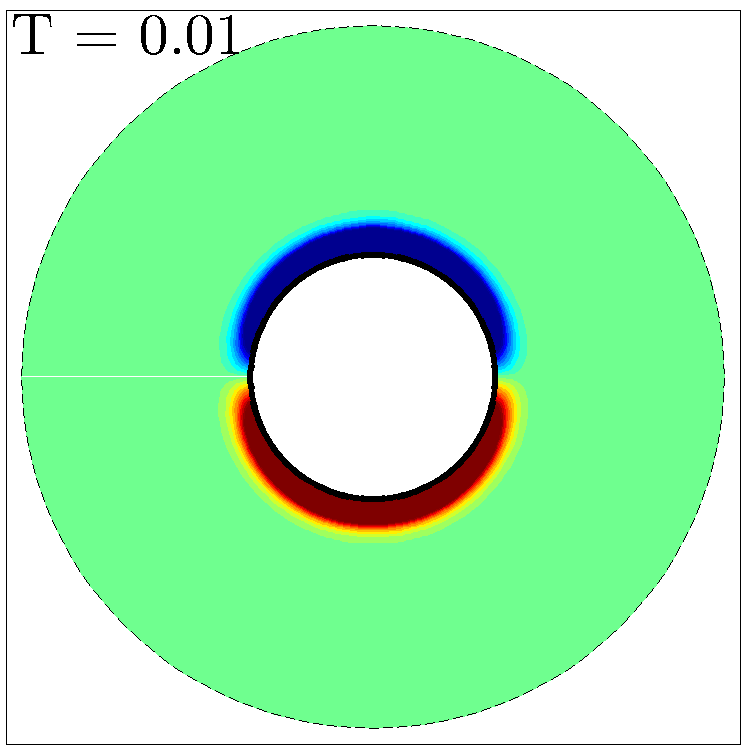
\includegraphics[width=6.5cm]{./Figures/results/static/vorticity_T0_01.pdf} & 
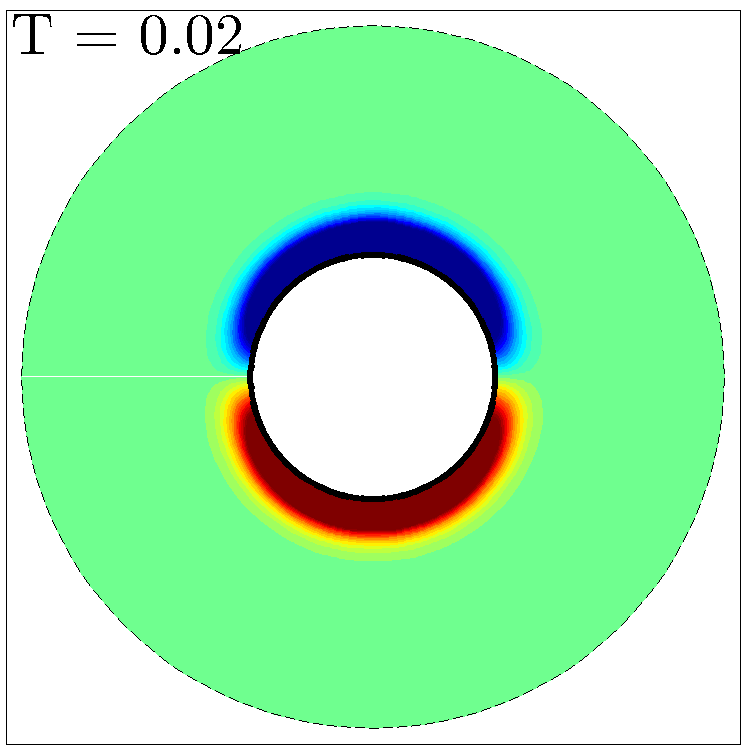
\includegraphics[width=6.5cm]{./Figures/results/static/vorticity_T0_02.pdf}  \\
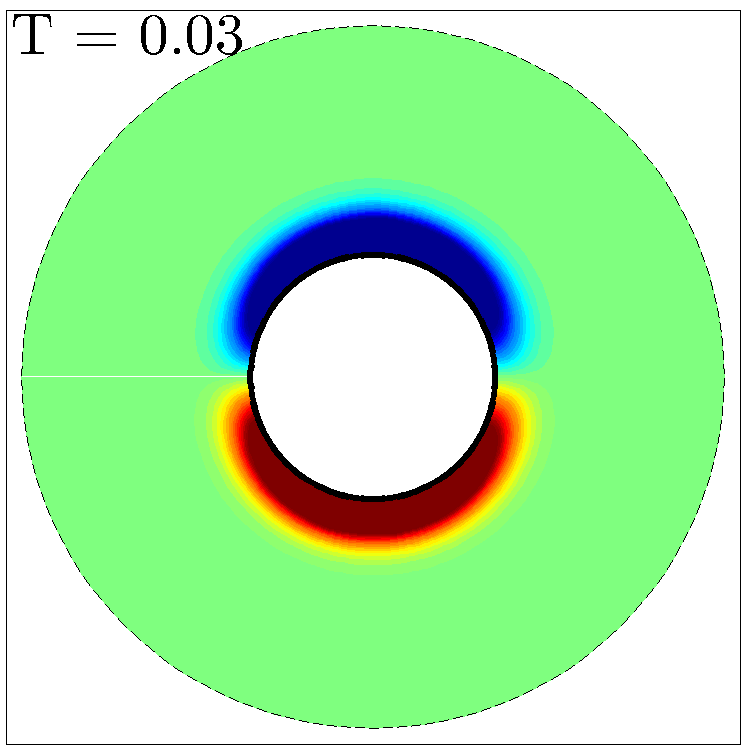
\includegraphics[width=6.5cm]{./Figures/results/static/vorticity_T0_03.pdf} & 
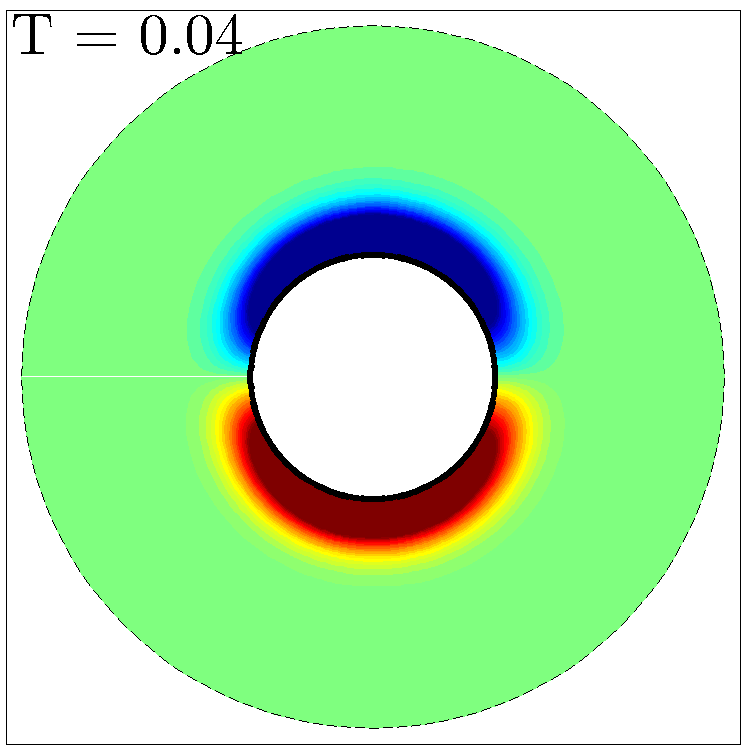
\includegraphics[width=6.5cm]{./Figures/results/static/vorticity_T0_04.pdf} \\
\tikz \draw (0,0) rectangle (2.5in, 2.5in) node[pos=0.1]{T = 0.05}; &
\tikz \draw (0,0) rectangle (2.5in, 2.5in) node[pos=0.1]{T = 0.06}; \\
\end{tabular}
\end{center}
\caption[Initial vorticity profile inside boundary layer]{Initial vorticity development inside boundary layer with time (boundary layer thickness magnified for visualization)}
\label{fig:InitialVorticity}
\end{figure}

\begin{figure}
\begin{center}
\begin{tabular}[t]{cc}
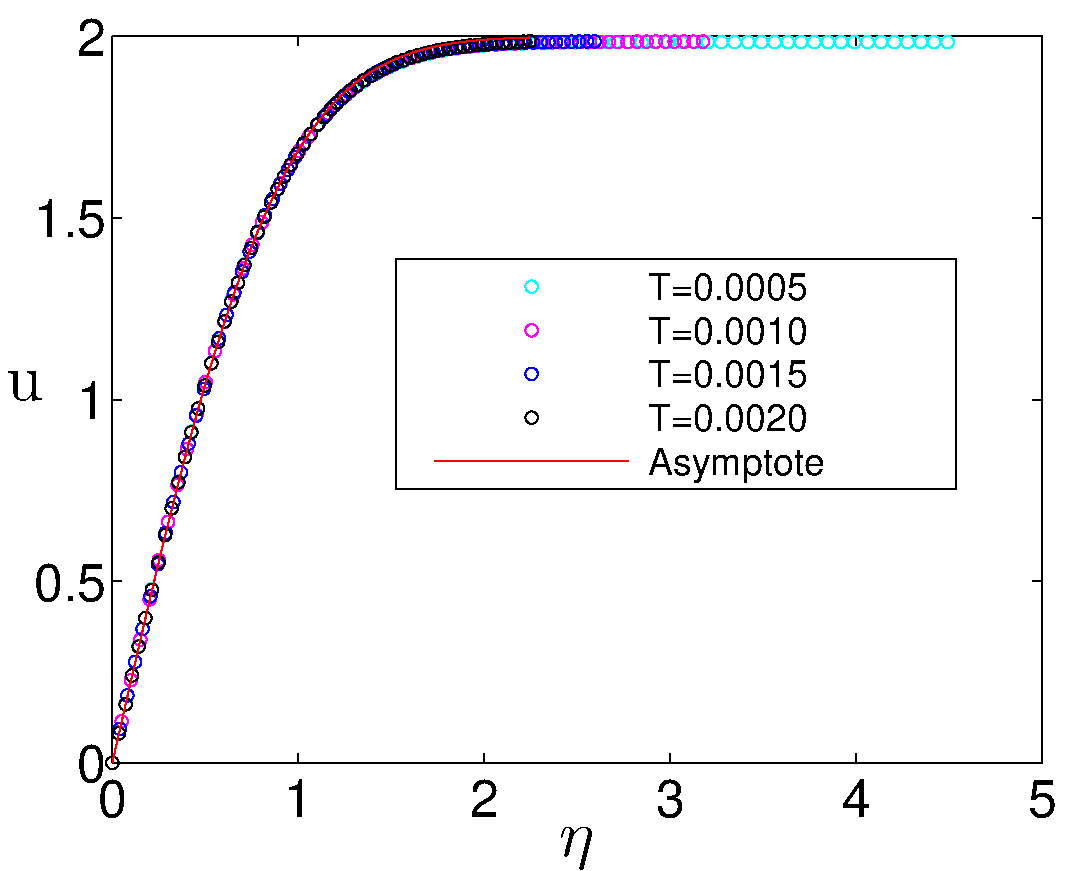
\includegraphics[width=12cm]{./Figures/results/static/u_asymptotic.pdf}  \\
(a) \\
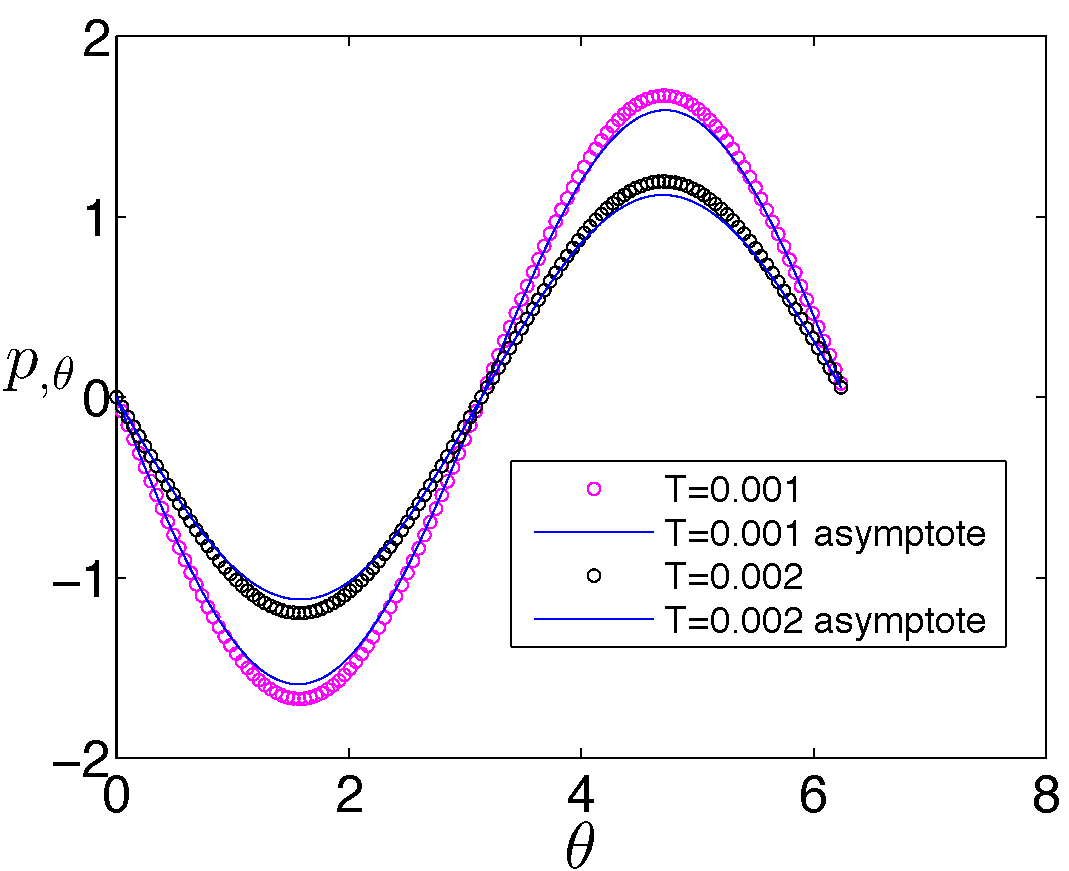
\includegraphics[width=12cm]{./Figures/results/static/p_asymptotic.pdf} \\
(b)
\end{tabular}
\end{center}
 \caption[Initial flow velocity and pressure compared with asymptotic solutions]{Initial flow properties compared with asymptotic solutions \cite{bar1975initial}. (a) shows that tangential velocity profiles at $\theta = \pi/2$ at different times collapse to the asymptotic solution; (b) shows the perturbation of pressure to inviscid case compared with the asymptotic solution.}
 \label{fig:InitialVelocity}
\end{figure}

\begin{figure}
\begin{center}
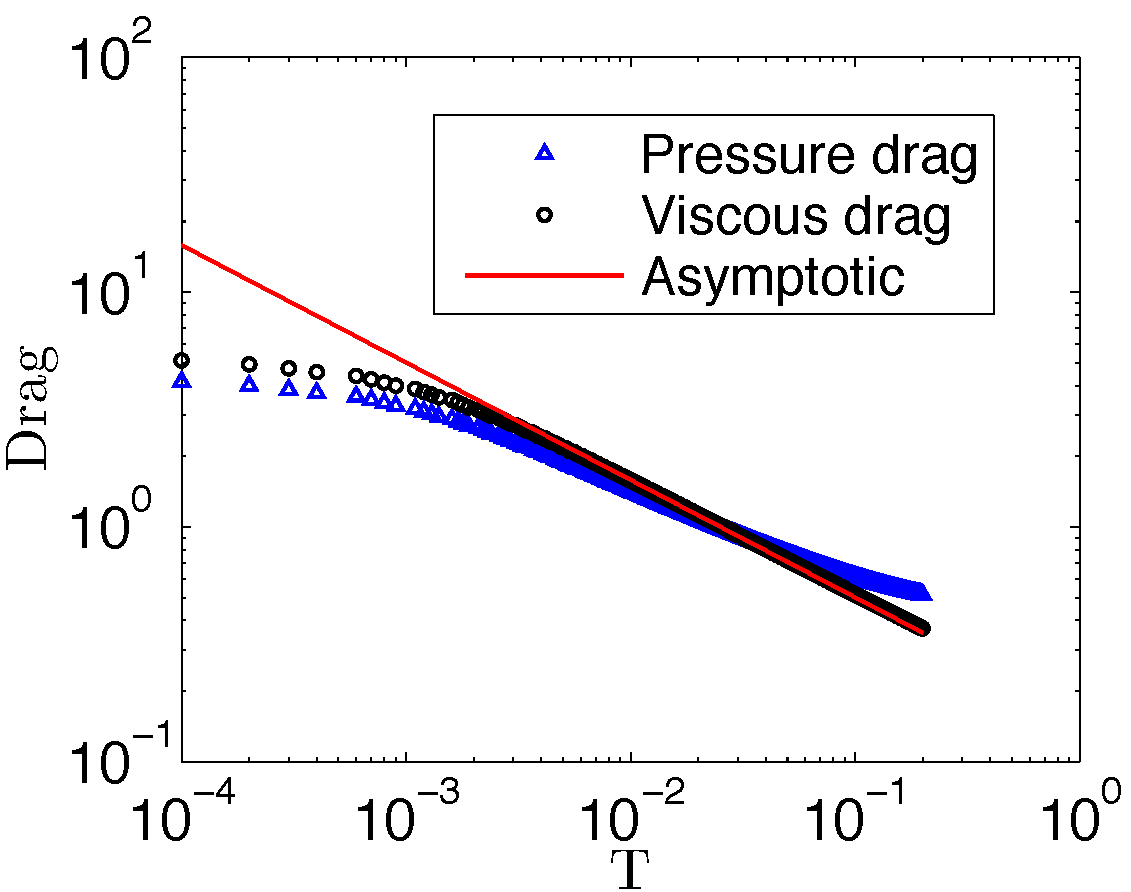
\includegraphics[width=12cm]{./Figures/results/static/InitialDrag.pdf}
\end{center}
 \caption[Initial flow properties compared with asymptotic solutions]{The drag coefficients at small time compared with asymptotic solution.}
 \label{fig:InitialDrag}
\end{figure}


One important feature which enriches the phenomena is the separation of flow from the cylinder surface.
The separation point is the point at which the vorticity vanishes and the vorticity gradient along the cylinder is negative, indicating a normal flow away from the cylinder. 
\noindent \\
\tikz \draw (0, 0) rectangle (\linewidth, 3in) node[pos=0.1]{Bar-Lev Yang with separation};
Figure \ref{fig:Separation} (a) shows that the layer of strong vorticity separates from the cylinder surface firstly close to the rear stagnation point and then the separation point moves upstream with time on both sides, which is quantitatively shown in Figure \ref{fig:SeparationAngle}. 
It is seen that the initial separation from the cylinder surface occurs at around $T = 0.4$, which agrees well with the asymptotic solution.
But it is seen that  compared to that of KL, our separation point moves away from the rear stagnation point slower.
Up to $T=6$, our boundary layer has not reached a steady state yet and hopefully after longer time our separation angle will approach the correct steady value.
On the other hand, with further diffusion and advection of vorticity, significant vorticity crosses our artificially chosen boundary $C$ of boundary layer and in our case discrete point vortices are shed into the outer region to represent the vorticity distribution as shown in Figure \ref{fig:Separation} (b).

\begin{figure}
 \begin{center}
 \begin{tabular}{cc}
 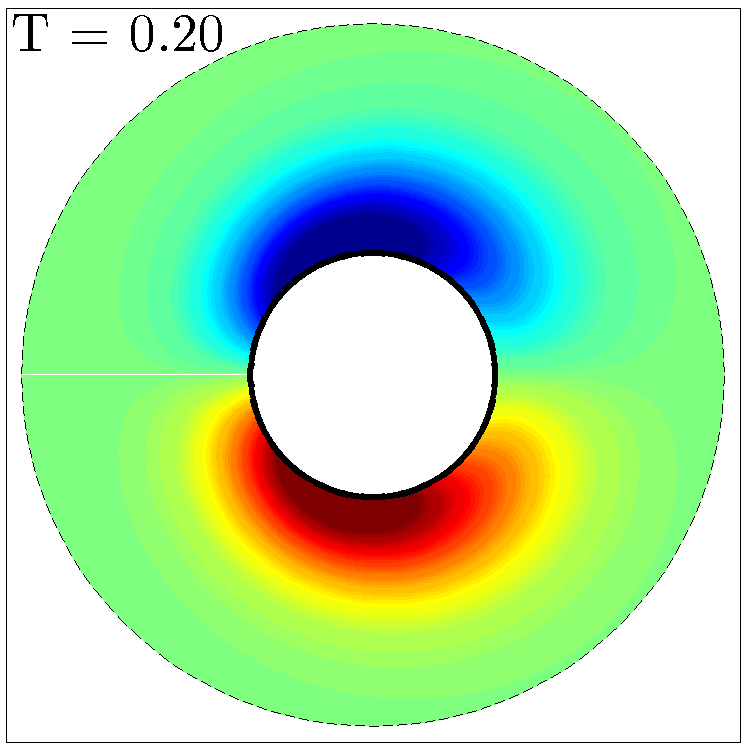
\includegraphics[width=5cm]{./Figures/results/static/vorticity_T0_20.pdf} &
 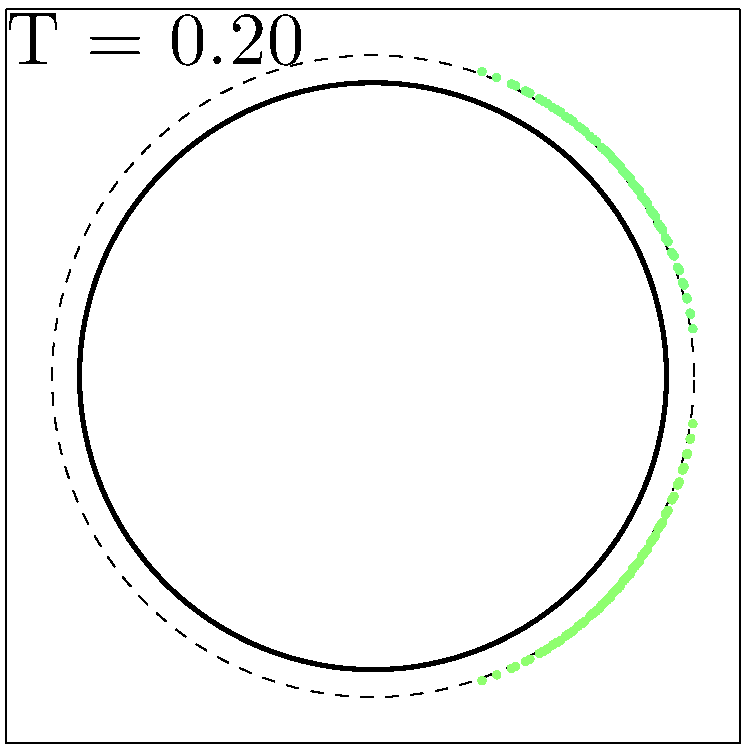
\includegraphics[width=5cm]{./Figures/results/static/vortices_T0_20.pdf}  \\
 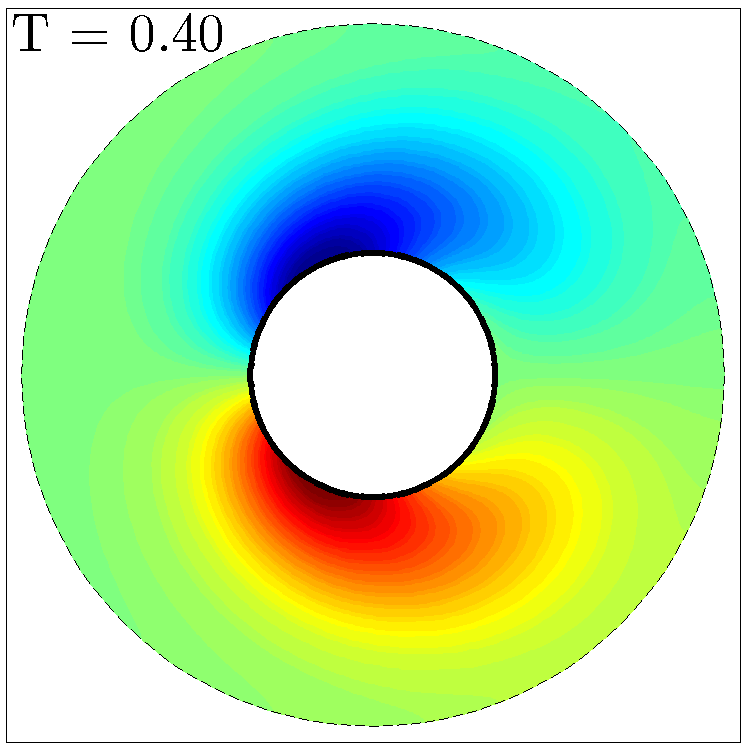
\includegraphics[width=5cm]{./Figures/results/static/vorticity_T0_40.pdf} &
 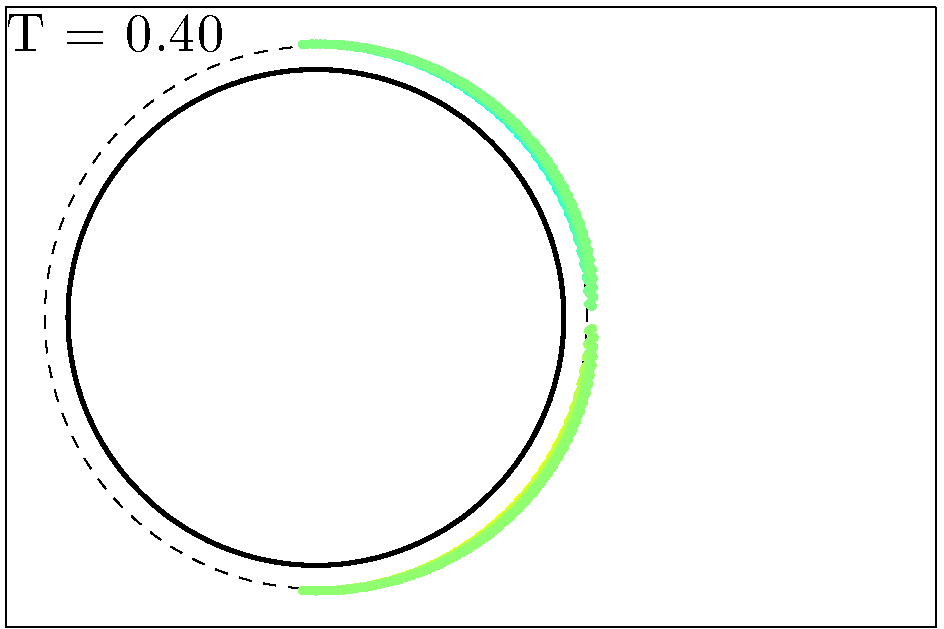
\includegraphics[width=5cm]{./Figures/results/static/vortices_T0_40.pdf}  \\
 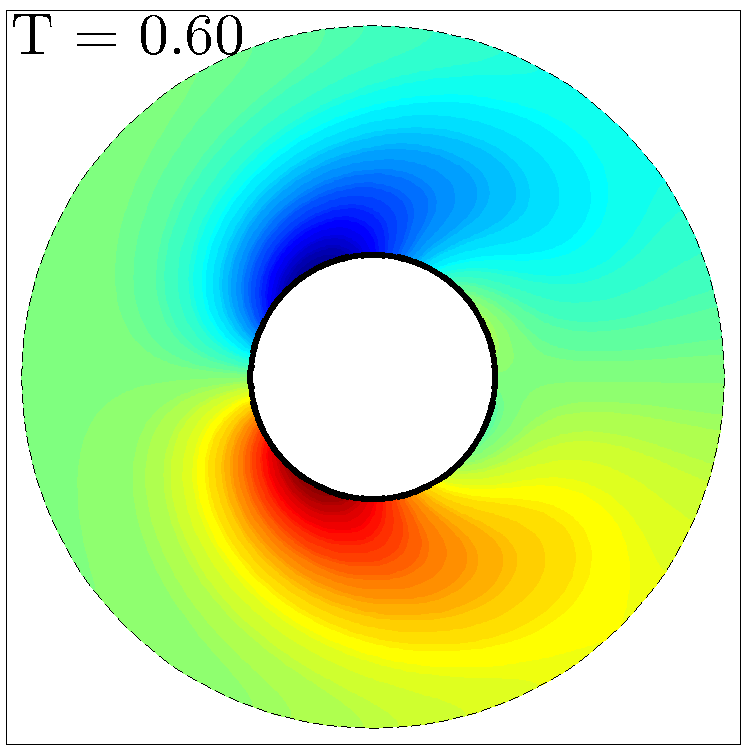
\includegraphics[width=5cm]{./Figures/results/static/vorticity_T0_60.pdf} &
 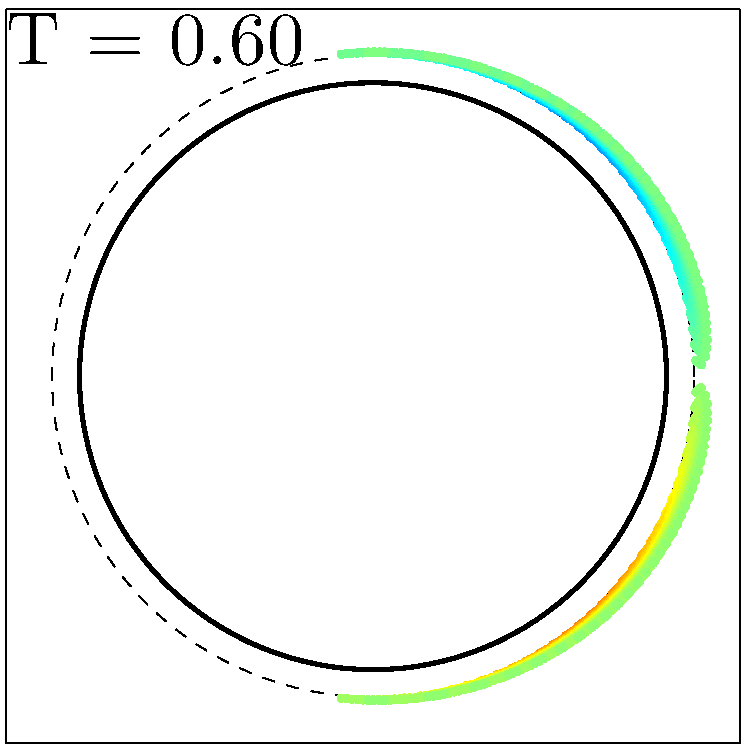
\includegraphics[width=5cm]{./Figures/results/static/vortices_T0_60.pdf}  \\
 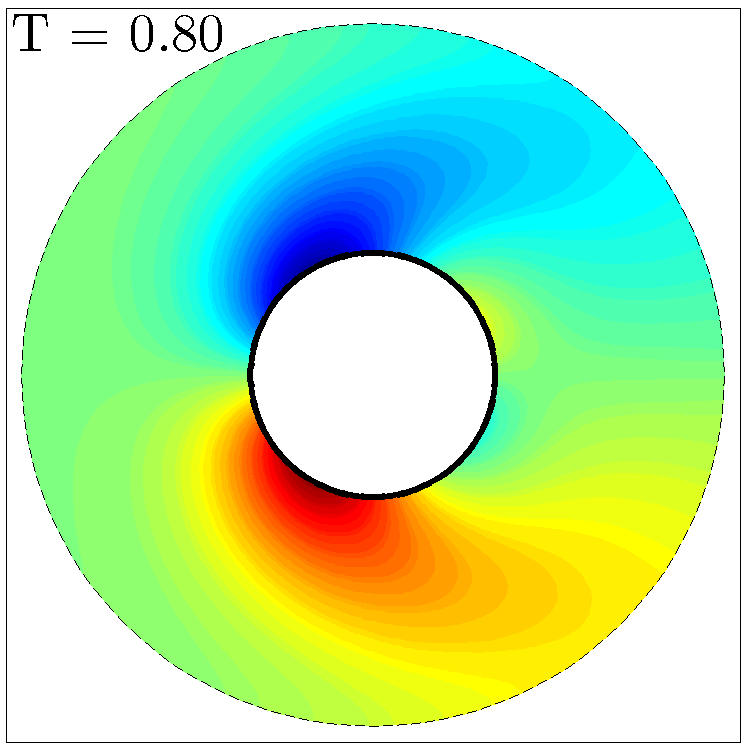
\includegraphics[width=5cm]{./Figures/results/static/vorticity_T0_80.pdf} &
 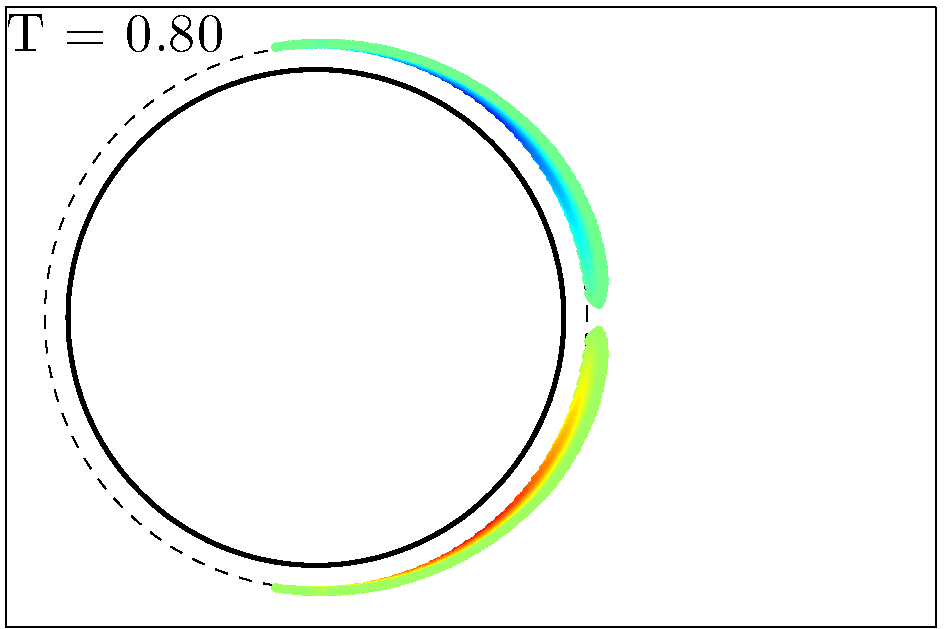
\includegraphics[width=5cm]{./Figures/results/static/vortices_T0_80.pdf}  \\
 (a) & (b)
\end{tabular}
\end{center}
 \caption[Flow separates]{The flow separates (a) as the vorticity gets diffused and convected away from the body. When significant vorticity reaches the edge of boundary layer, certain amount of point vortices are shed into the outer region (b). }
 \label{fig:Separation}
\end{figure}

\begin{figure}
 \begin{center}
 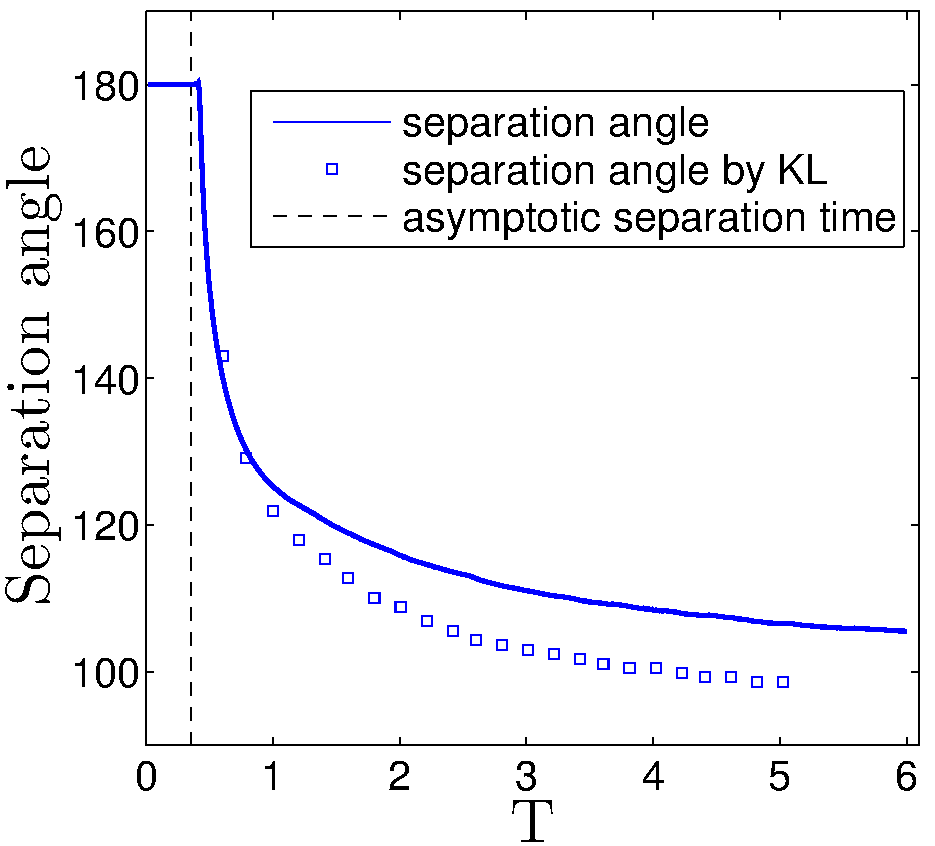
\includegraphics[width=12cm]{./Figures/results/static/separation_angle.pdf}
 \end{center}
 \caption[Evolution of separation angle]{The time progression of separation angle compared with the direct numerical simulation result by KL.}
 \label{fig:SeparationAngle}
\end{figure}


The later-time progression of the vorticity field is shown in Fig \ref{fig:Wake}, with comparison to the DNS results using vortex methods.
At this stage of moderate time, the wake remains symmetric,  characterized by one primary vortex and one small secondary vortex on both upper and lower half planes. 
Fed by a thick shear layer connected to the body, each primary vortex is passively convected by the free-stream velocity.
Initially the layer that feeds the primary vortex changes angle of orientation in respect to the body, but it seems that a stable configuration is in place later.
As the secondary vortex grows, it penetrates the primary vortex but it is always confined and never able to reach the outer irrotational flow field.
Compared to the result by KL, the feeding vorticity layer is spanning a smaller angle relative to the body, indicating a little bit weaker vortex shedding. 
The quantitative parameter to observe here is still the drag coefficient shown in Fig \ref{fig:Drag}.
Our viscous drag agrees well with the DNS result, also following the asymptotic solution.
On the other hand, our model gives the pressure drag with the same trend as that by KL, but quantitatively our pressure drag is relatively higher, which is possibly also because our vortex shedding is not as strong as theirs. 

\begin{figure}
 \begin{center}
 \begin{tabular}{cc}
 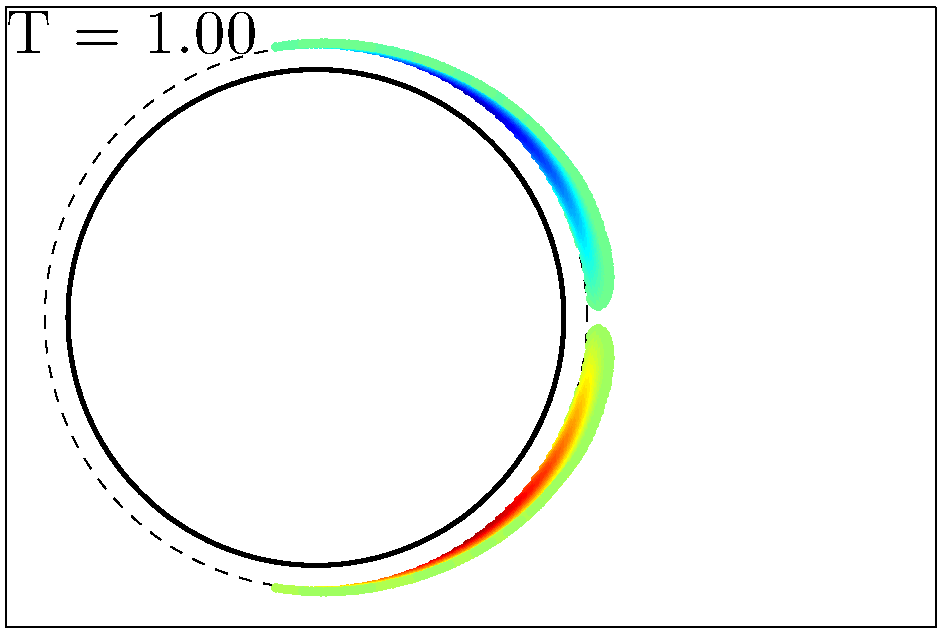
\includegraphics[width=6cm]{./Figures/results/static/vortices_T1_00.pdf}  &
 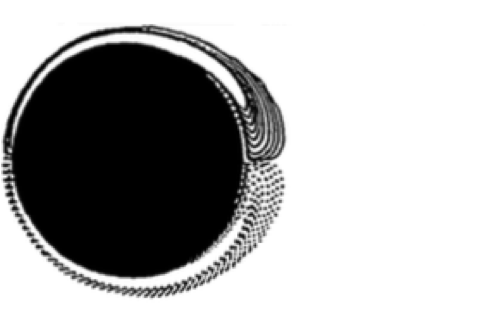
\includegraphics[width=6cm]{./Figures/results/static/KOU_Re1000_T1.png}  \\
 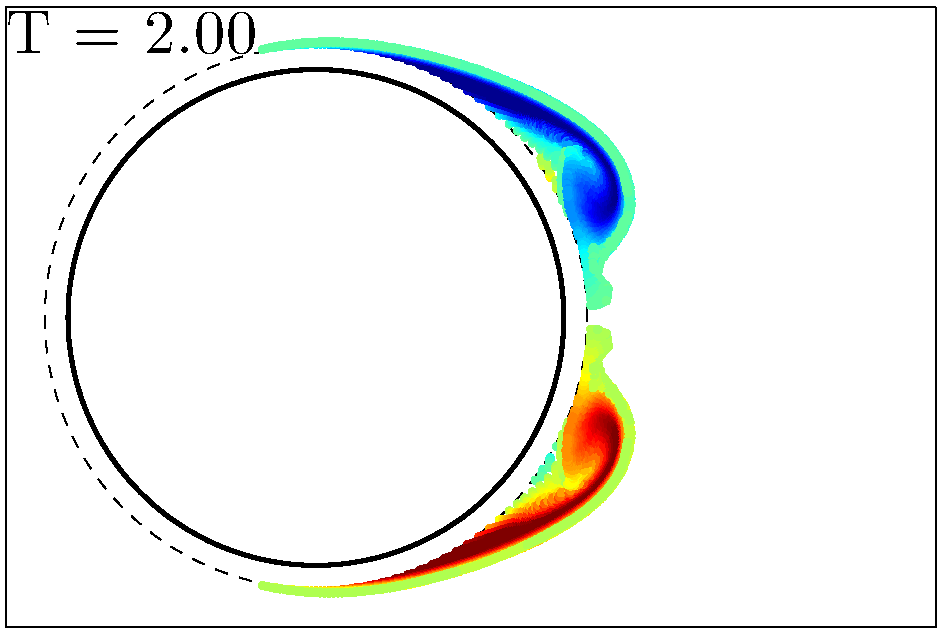
\includegraphics[width=6cm]{./Figures/results/static/vortices_T2_00.pdf}  &
 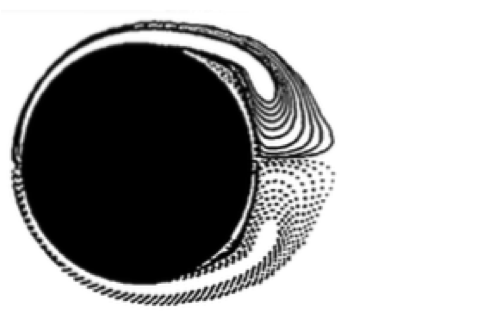
\includegraphics[width=6cm]{./Figures/results/static/KOU_Re1000_T2.png}  \\
 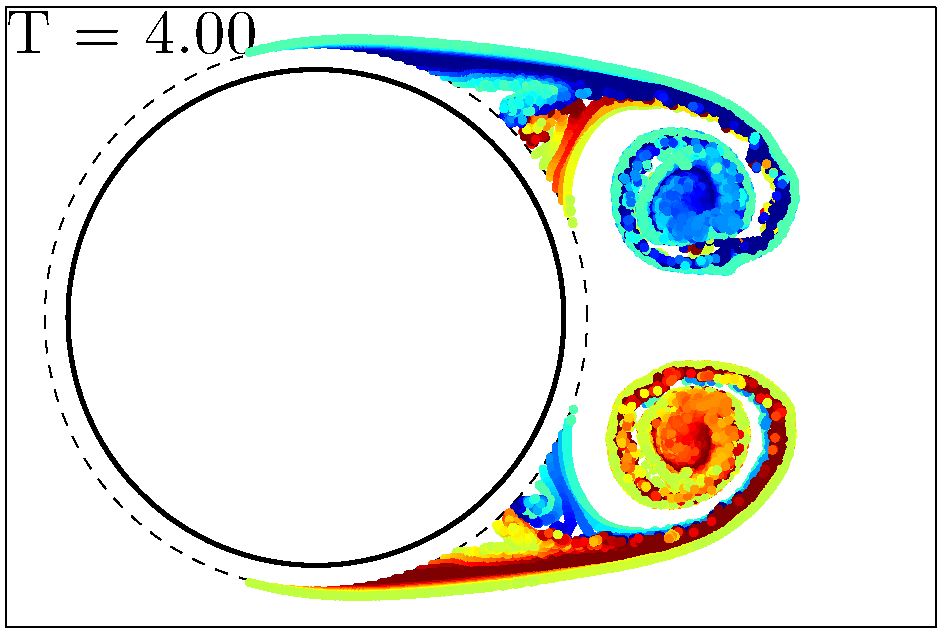
\includegraphics[width=6cm]{./Figures/results/static/vortices_T4_00.pdf}  &
 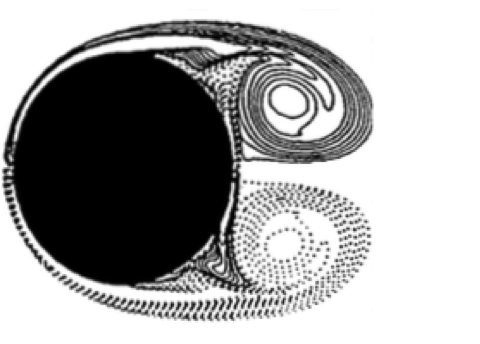
\includegraphics[width=6cm]{./Figures/results/static/KOU_Re1000_T4.png}  \\
 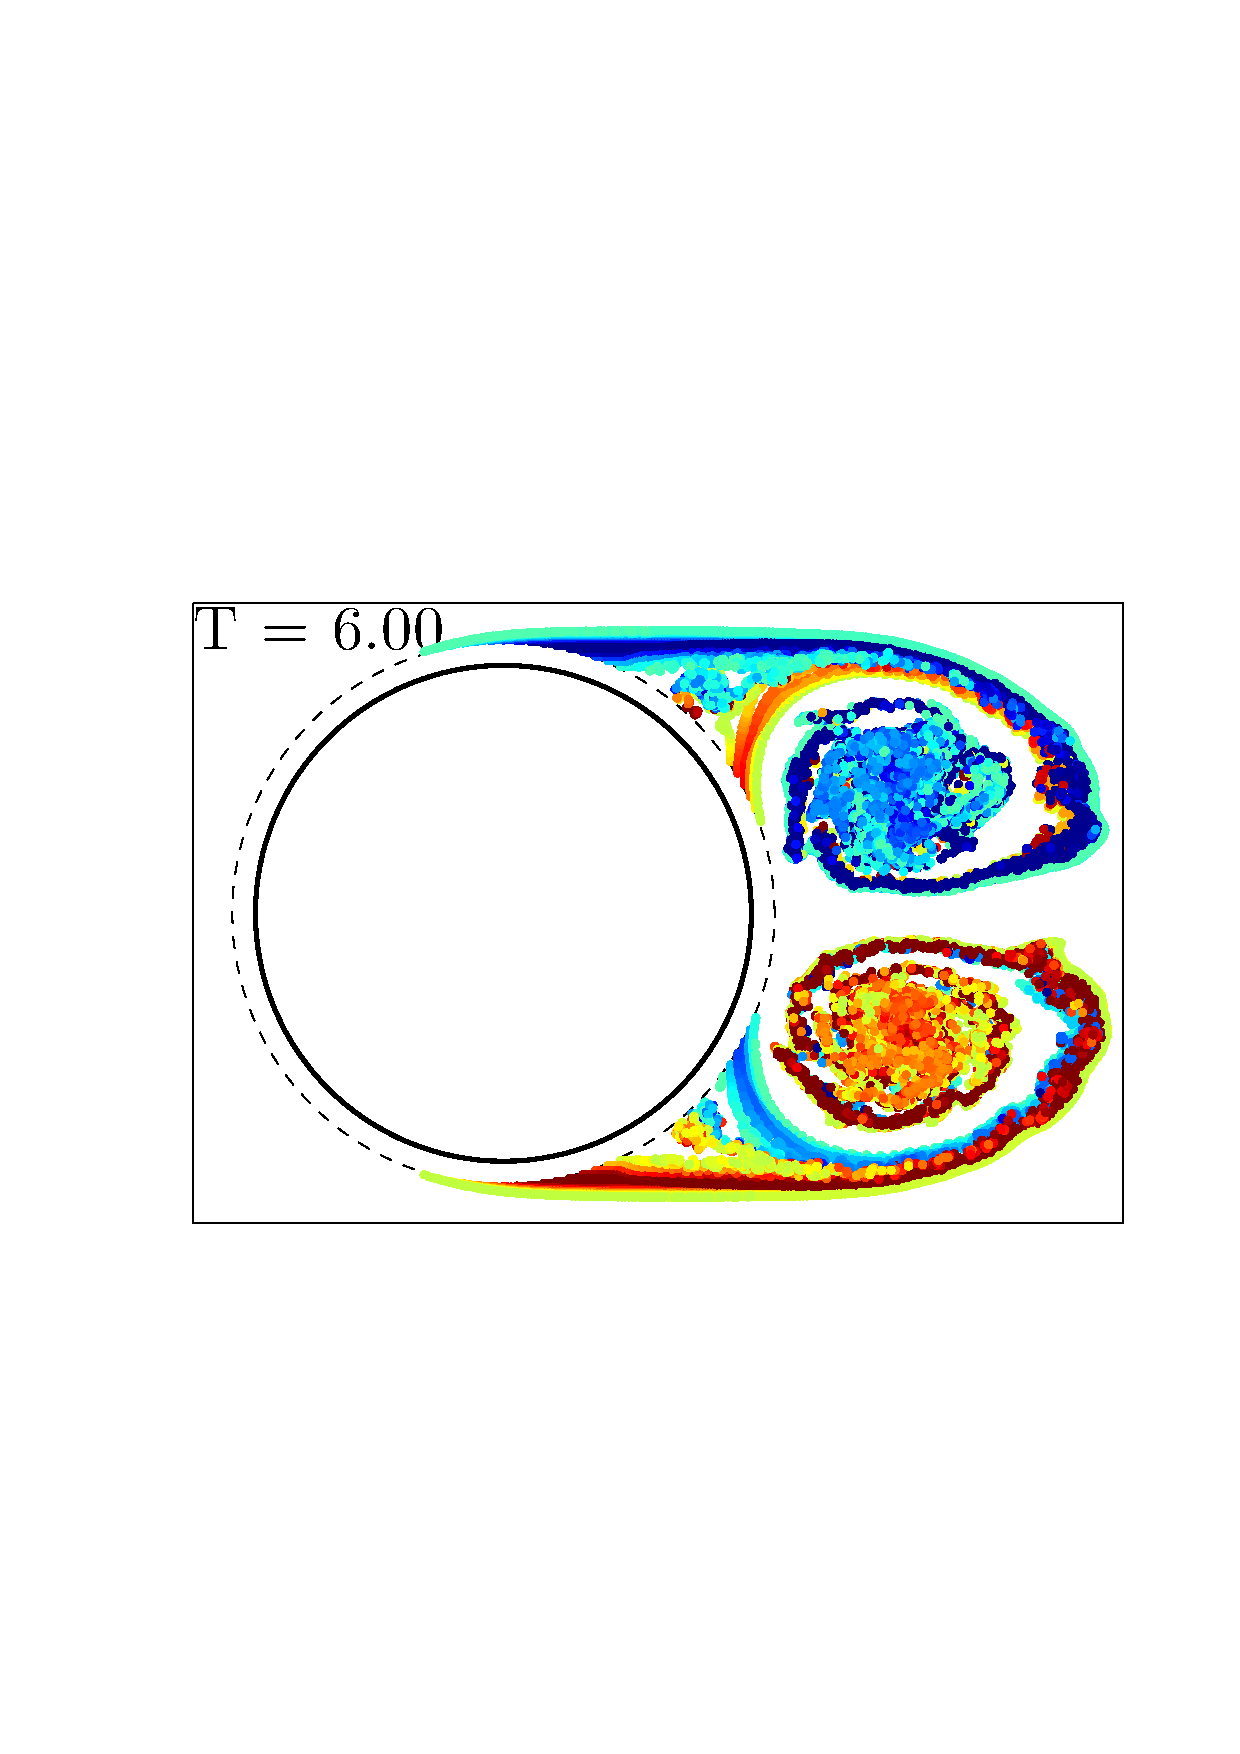
\includegraphics[width=6cm]{./Figures/results/static/vortices_T6_00.pdf}  &
 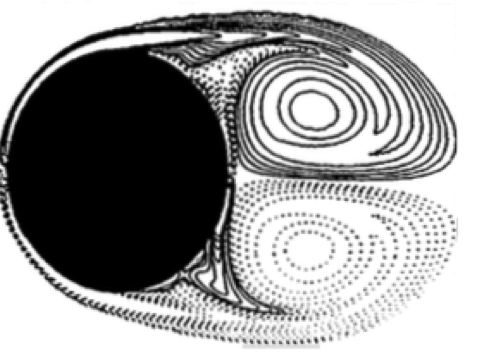
\includegraphics[width=6cm]{./Figures/results/static/KOU_Re1000_T6.png}  \\
 (a) & (b) \\
 \end{tabular}
\end{center}
 \caption[Vortex shedding pattern in the wake]{The progression of vortex shedding pattern (a) with comparison to direct numerical simulation result by vortex methods (b). }
 \label{fig:Wake}
\end{figure}

\begin{figure}
\begin{center}
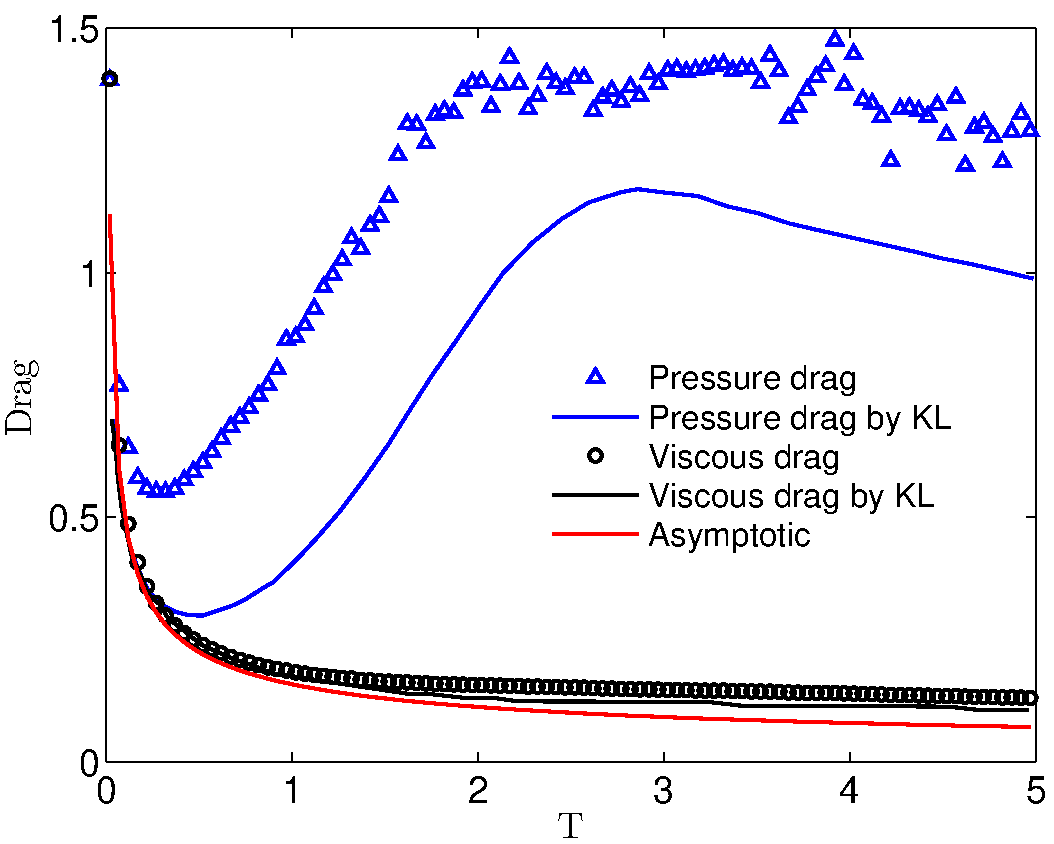
\includegraphics[width=12cm]{./Figures/results/static/Drag.pdf}
\end{center}
\caption[Drag coefficient]{The drag coefficient compared with direct numerical simulation results and small-time asymptotic.}
\label{fig:Drag}
\end{figure}


Last but not least, although Prandtl's boundary layer approximation is expected to fail at the separation point, we still believe that our model can capture the vortex shedding based on our arguments presented in the previous section (Rationale). 
The total circulation in the upper-half plane computed with different boundary layer thickness $c/\sqrt{Re}$ is shown in Fig \ref{fig:Circulation}.
It is seen that our computed circulation qualitatively follows the same trend as the result by computational fluid dynamics (CFD).
Besides, it confirms  that within certain range the exact location of the interface $C$ does not affect the total circulation significantly, but just determines where we switch over the representation of flows.

\begin{figure}
\begin{center}
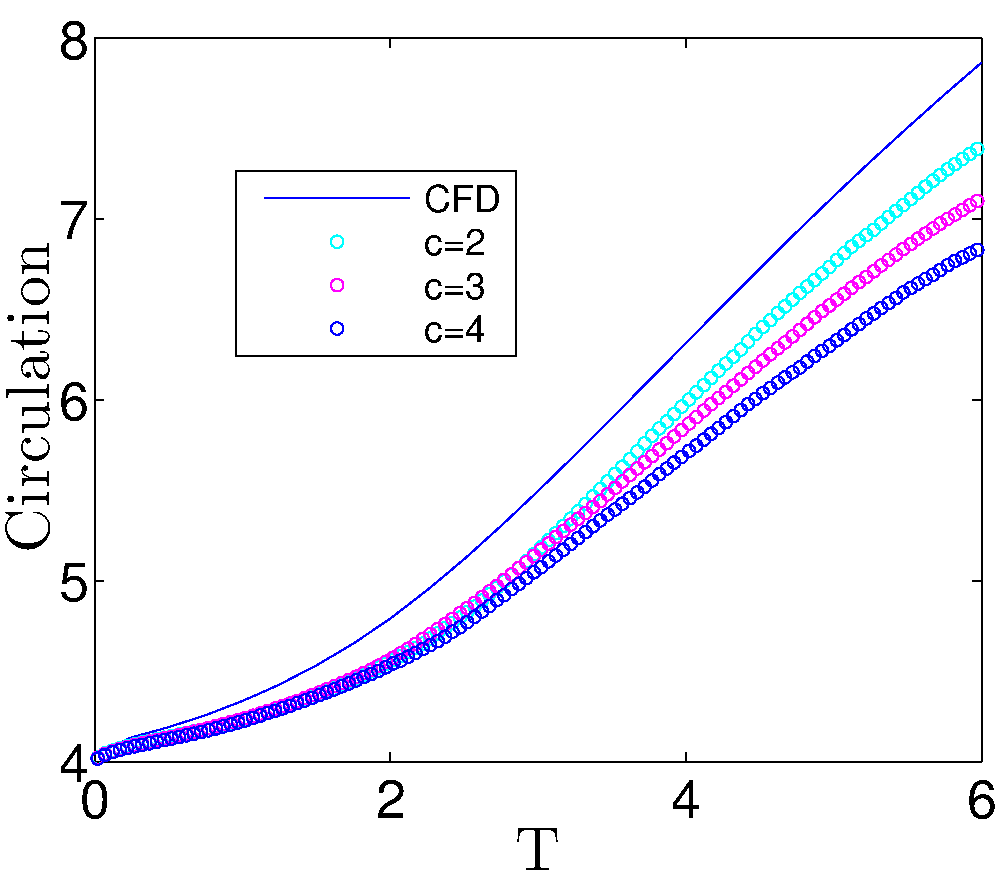
\includegraphics[width=12cm]{./Figures/results/static/Circulation.pdf}
\end{center}
\caption[Total circulation in the upper-half plane]{Total circulation in the upper-half plane calculated with different boundary layer thickness $c/\sqrt{Re}$, compared with CFD result.}
\label{fig:Circulation}
\end{figure}


\subsection{Impulsively started flow past a rotating cylinder}


\begin{figure}
 \begin{center}
 \begin{tabular}{cc}
 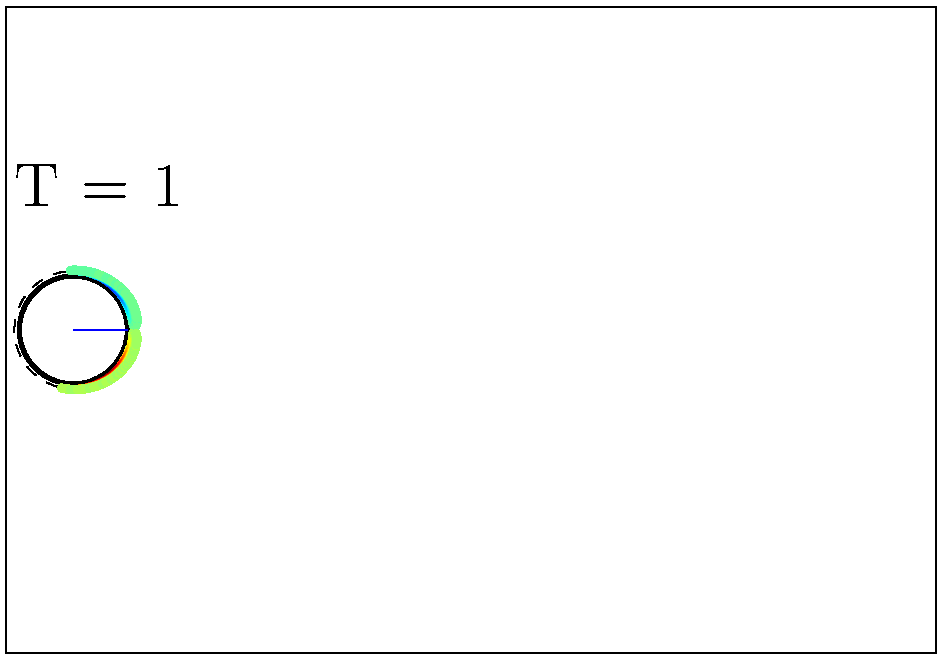
\includegraphics[height=4cm]{./Figures/results/rotating/vortices_T1.pdf}  &
 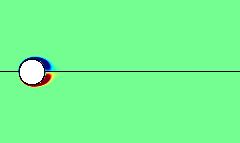
\includegraphics[height=4cm]{./Figures/results/rotating/T_1.png}  \\
 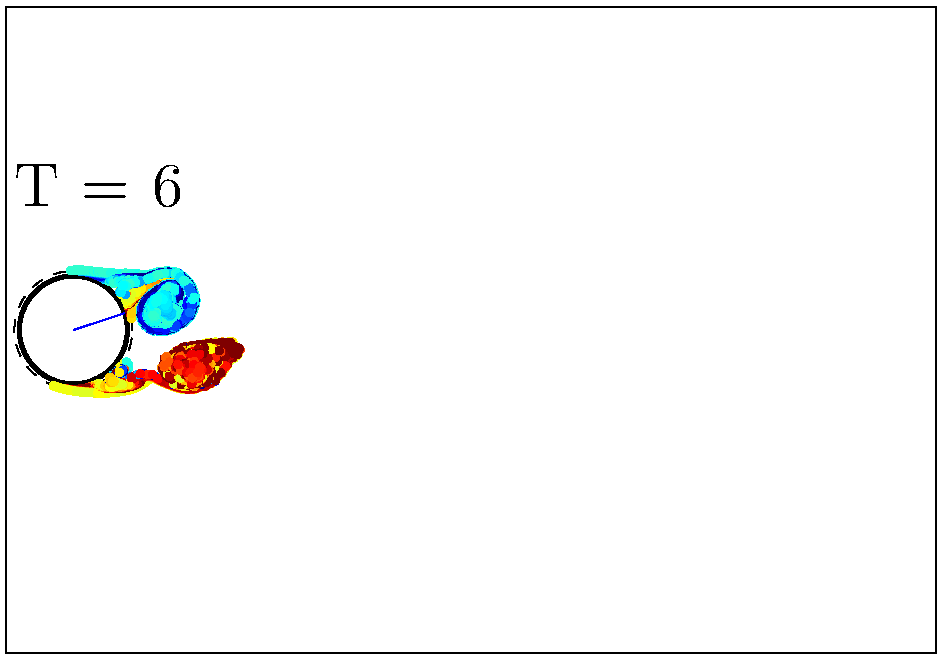
\includegraphics[height=4cm]{./Figures/results/rotating/vortices_T6.pdf}  &
 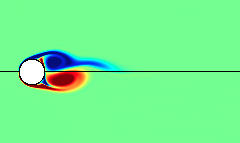
\includegraphics[height=4cm]{./Figures/results/rotating/T_6.png}  \\
 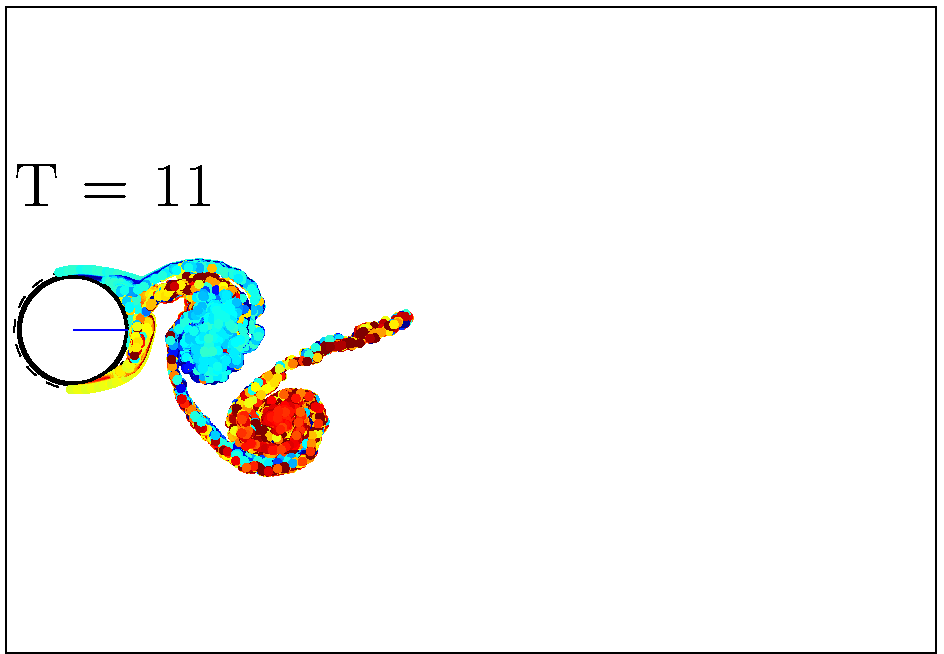
\includegraphics[height=4cm]{./Figures/results/rotating/vortices_T11.pdf}  &
 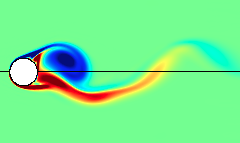
\includegraphics[height=4cm]{./Figures/results/rotating/T_11.png}  \\
 (a) & (b) \\
 \end{tabular}
\end{center}
 \caption[Vortex shedding pattern around a sinusoidally rotating cylinder]{The progression of vortex shedding pattern (a) with comparison to direct numerical simulation result by vortex methods (b). }
 \label{fig:RotatingWake1}
\end{figure}

\begin{figure}
 \begin{center}
 \begin{tabular}{cc}
 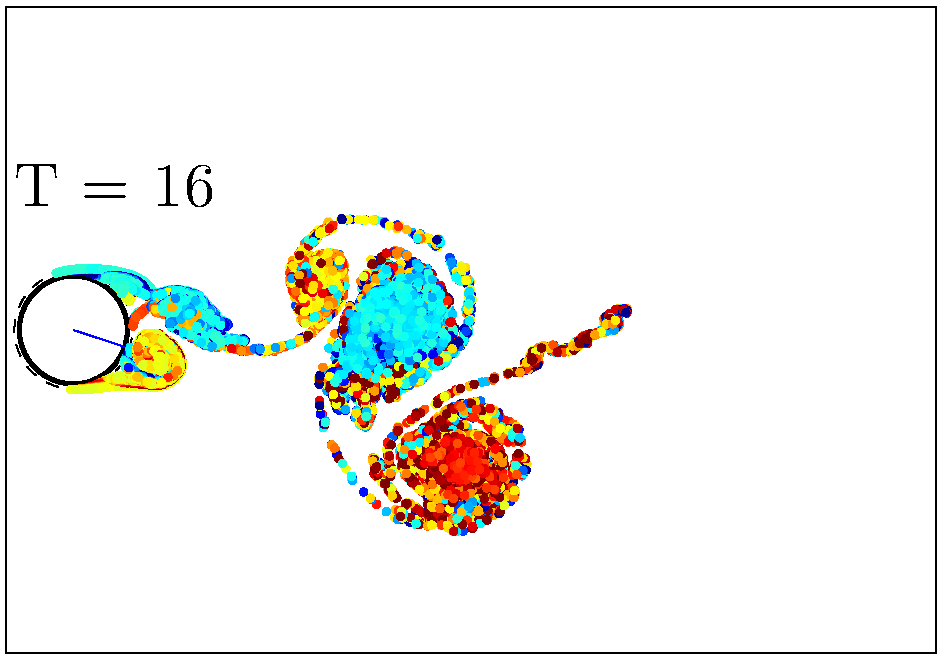
\includegraphics[height=4cm]{./Figures/results/rotating/vortices_T16.pdf}  &
 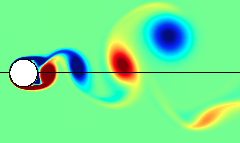
\includegraphics[height=4cm]{./Figures/results/rotating/T_16.png}  \\
 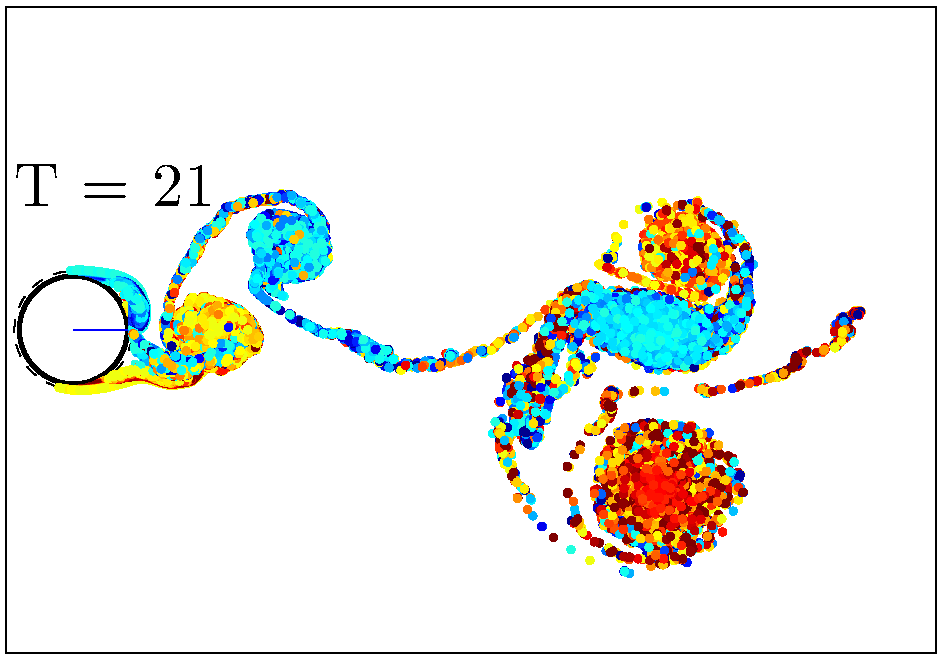
\includegraphics[height=4cm]{./Figures/results/rotating/vortices_T21.pdf}  &
 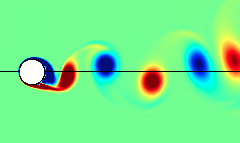
\includegraphics[height=4cm]{./Figures/results/rotating/T_21.png}  \\
 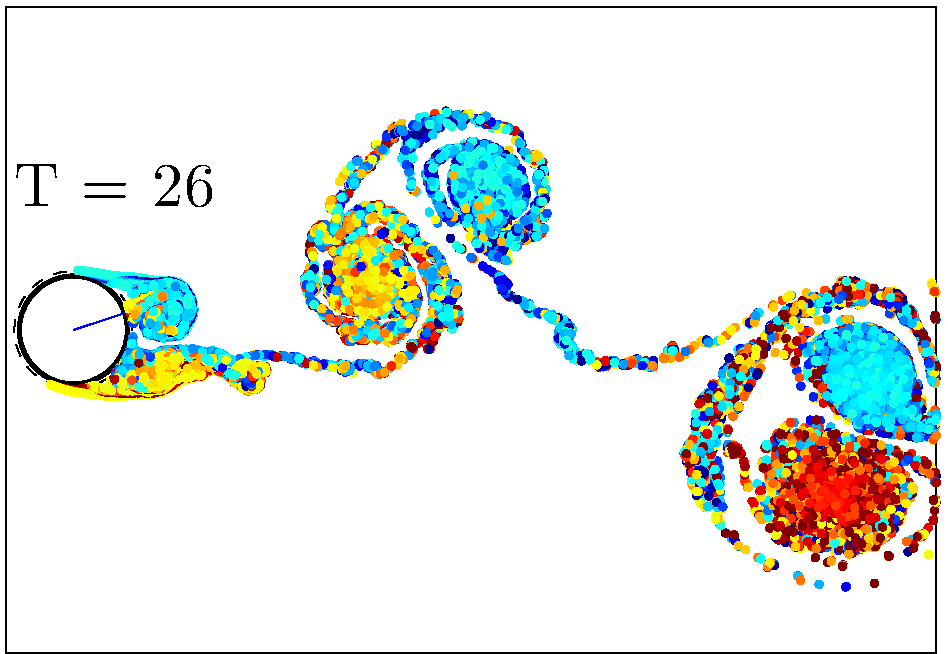
\includegraphics[height=4cm]{./Figures/results/rotating/vortices_T26.pdf}  &
 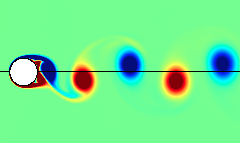
\includegraphics[height=4cm]{./Figures/results/rotating/T_26.png}  \\
 (a) & (b) \\
 \end{tabular}
\end{center}
 \caption[Vortex shedding pattern around a sinusoidally rotating cylinder]{The progression of vortex shedding pattern (a) with comparison to direct numerical simulation result by vortex methods (b). }
 \label{fig:RotatingWake2}
\end{figure}

